%!TEX encoding = UTF-8 Unicode
%!TEX program = xelatex

\documentclass[bachelor]{ustcthesis}
% bachelor|master|doctor
\usepackage{ustcextra}
\graphicspath{{figures/}}
\bibliographystyle{ustcauthoryear}
% \bibliographystyle{ustcnumerical}

\renewpagestyle{front}[\zihao{-5}]{
    \sethead{}{软件工程作业管理系统概要设计}{}
    \setfoot{}{\thepage}{}
    \headrule
}
\renewpagestyle{main}[\zihao{-5}]{
    \sethead{}{软件工程作业管理系统概要设计}{}
    \setfoot{}{\thepage}{}
    \headrule
}
\newcommand{\HRule}{\rule{\linewidth}{0.5mm}}
\newcommand{\tabincell}[2]{\begin{tabular}{@{}#1@{}}#2\end{tabular}}

\begin{document}



\begin{titlepage}
\begin{center}
~\\[5cm]
\HRule \\[0.4cm]
{\huge \bfseries 软件工程作业管理系统\\概要设计}\\[0.4cm]
\HRule \\[1.5cm]

\begin{tabular}{ccc}
  & 人员 & 日期 \\ 
拟制 & 张三\ 李四\ 王五 & yyyy-mm-dd \\ 
评审人 & • & yyyy-mm-dd \\ 
批准 & • & yyyy-mm-dd \\ 
签发 & • & yyyy-mm-dd \\ 
\end{tabular} 

\end{center}
\end{titlepage}



\frontmatter
\begin{abstract}
本文是软件工程需求规格说明书模板,修改自于中国科学技术大学本硕博毕业论文 \LaTeX{} 模板示例文件,该模板由
zepinglee和seisman创建,遵循中国科学技术大学的论文写作规范,适用于撰写学士、硕士和博士学位论文。

本文档最后一章演示如何使用 \LaTeX{} 的一些基本命令以及本模板提供的一些特殊功能,
模板的选项及详细用法请参考模板说明文档 ustcthesis.pdf。请在提交之前把最后一掌实例注释掉。

\keywords{软件工程\zhspace{} 中国科学技术大学\zhspace{} 学位论文\zhspace{} \LaTeX{}~通用模板\zhspace{} 学士\zhspace{}
硕士\zhspace{} 博士\zhspace{} 示例文档\zhspace{} 模板说明文档}

\begin{table}[htbp]
\centering
\caption{缩略词清单} \label{tab:simpletable}
\begin{tabular}{|c|c|c|}
    \hline
    缩略语 & 英文全名 & 中文解释 \\
    \hline
    c & d & e\\
    \hline
\end{tabular}
\end{table}

\end{abstract}

\tableofcontents
\listoffigures
\listoftables
% \listofalgorithms  % 算法索引,如不需要,可直接注释掉本行
% \begin{notation}

%\centering
%XX 软件需求规格说明书

%关键词:能够体现文档描述内容主要方面的词汇。
 
%摘要:


\centering
\begin{tabular}{rl}
$\ln x$ & natural logarithm $\log_ex$ \\
$\log x$ & common logarithm $\log_{10}x$ \\
$x\ \mathrm{mod}\ y$ & remainder \\
\end{tabular}

\end{notation}


\mainmatter
\chapter{简介}
\section{目的}


本需求文档主要为软件开发者所制作,意在指明即时通讯软件系统(以下简称通讯系统)的开发需求和具体实现方向。

本文档还可作为软件开发过程中的备案,为后续需求的提出给出参考。此外,非软件开发者可以将这个文件视为我们的即时通讯系统的开发纲要。

\section{范围}


本文档主要包括
\begin{enumerate}
	\item 通讯系统的总体概述
	
	\item 通讯系统的具体需求
	
	\item 通讯系统的设计约束
	
	\item 通讯系统的软件质量特性
	
	\item 通讯系统的其它要求
	
	\item 通讯系统的依赖关系
	
	\item 通讯系统的需求分级
	
	\item 其它待定问题 
\end{enumerate}

对应的,本文档除去上述内容之外,不会包含设计理念、实现方法、开发过程等细节上的问题。

\chapter{任务概述}
本系统的目标是实现一个xxx系统,包括客户端、服务器端两个部分。

客户端面向xxx用户,为用户提供xx和xx服务。

\section{目标}
实现xxx系统,实现需求规格说明书中所描述的xx功能、xxx功能和xxx功能,并且保证系统的健壮性和数据安全。

\section{开发与运行环境}

\subsection{开发环境的配置}
\begin{table}[htbp]
\centering
\caption{开发环境的配置} \label{tab:development-environment}
\begin{tabular}{|c|c|c|}
    \hline
    类别 & 标准配置 & 最低配置 \\
    \hline
    计算机硬件 & \tabincell{c}{基于x86结构的CPU\\ 主频>=2.4GHz\\ 内存>=8G\\ 硬盘>=200G} & \tabincell{c}{基于x86结构的CPU\\ 主频>=1.6GHz\\ 内存>=512M\\ 硬盘>=2G} \\
    \hline
    计算机软件 & \tabincell{c}{Linux (kernel version>=4.10)\\ GNU gcc (version>=6.3.1)} & \tabincell{c}{Linux (kernel version>=3.10)\\ GNU gcc (version>=5.4)} \\
    \hline
    网络通信 & \tabincell{c}{至少要有一块可用网卡\\ 能运行IP协议栈即可} & \tabincell{c}{至少要有一块可用网卡\\ 能运行IP协议栈即可} \\
    \hline
    其他 & 采用MySQL数据库 & 采用MySQL数据库 \\
    \hline
\end{tabular}
% \note{这里是表的注释}
\end{table}

\section{需求概述}
功能需求包括:


\section{条件与限制}
本节至少要与需求说明文档中相关章节相一致。

\chapter{总体设计}
\section{软件描述}
系统包括前台和后台两个部分。

前台主要功能是:
给用户提供交互的接口,用于各种功能。
后台主要功能是:
处理用户发出的请求,后台记录用户产生的数据等等。

\section{处理流程}
\subsection{总体流程}
此处应当有一个图和对应的描述。

\subsection{系统基本流程}
此处应当有一个图和对应的描述。

\subsection{客户端基本流程}
用户登录-> 显示消息列表 -> 选择具体功能 -> 聊天或者等待或者退出

\subsection{服务器端基本流程}


\subsection{功能1具体流程}


1. 用户注册或登录

在打开应用的第一个页面,会有用户名和密码的输入框,在正确输入用户名和密码之后点击sign in便可以登入。或者可以点击另外一个sign up的按钮,
创建一个用户名没有重复的账户之后输入验证码便会通过,服务器数据更新之后便可以使用这个新的账户登录。


\subsection{功能2具体流程}

2. 单人聊天

已登录用户会进入一个新的功能页面(称为主页面)。在主页面首先在消息列表中选择的已有对话,或者在联系人列表中选择联系人新建对话。

\subsection{功能3具体流程}
3. 大厅聊天

已登录用户在主页面选择大厅聊天,输入任何自己想说的并发送即可。要注意的是,在大厅说的所有话都会被所有在线用户看到。



\section{功能结构设计}
\subsection{整体结构}
此处应当有一个图和对应的描述。系统如果像微内核那样,划分成核心模块和若干个子系统,此处应当有图示及说明,然后后续几个节应当描述这几个子系统。如果系统像宏内核,那应当说明有哪些紧密联系的模块,并在后续几个节内描述这些模块。

\subsection{用户端结构}
此处应当有一个图和对应的描述。这只是举个例子。可能的内容包括用户端的具体模块、耦合情况等。

\subsection{服务器端结构}
此处应当有一个图和对应的描述。这只是举个例子。

\subsection{后台数据库维护模块结构}
此处应当有一个图和对应的描述。这只是举个例子。



\section{功能需求与程序代码的关系}
[此处指的是不同的需求分配到哪些模块去实现。可按不同的端拆分此表]
\begin{table}[htbp]
\centering
\caption{功能需求与程序代码的关系表} \label{tab:requirement-module}
\begin{tabular}{|c|c|c|c|}
    \hline
    · & 模块1 & 模块2 & 模块3 \\
    \hline
    需求1 & · & Y & · \\
    \hline
    需求2 & · & Y & · \\
    \hline
    需求3 & · & Y & · \\
    \hline
    需求4 & Y & · & · \\
    \hline
    需求5 & · & · & Y \\
    \hline
\end{tabular}
\note{各项功能需求的实现与各个程序模块的分配关系}
\end{table}
\chapter{接口设计}
\section{外部接口}
比如说需要用到支付宝等外部支付系统,接口应当如何封装。

\subsection{支付宝接口}
详细讲述不同的接口(查询状态、支付交易、获取回执等)

\section{内部接口}
内部模块/系统之间的交互的接口。
\chapter{数据结构设计}
\section{逻辑结构设计}
\subsection{用户管理系统数据结构设计}
用户信息
	\begin{itemize}  	
		\item 用户名 varchar(48)
		\item 密码盐 char(10)
		\item MD5值 char(32)
	\end{itemize}
用户关系信息
	\begin{itemize}  	
		\item 用户名1 varchar(48)
		\item 用户名2 varchar(48)
\end{itemize}
离线消息信息
	\begin{itemize}
		\item 发送用户 varchar(48)
		\item 接收用户 varchar(48)
		\item 信息     varchar(1024)
		\item 发送时间 datetime
	\end{itemize}	
\subsection{客户端数据结构}
数据包
	\begin{itemize}
		\item 消息类型 MessageType
		\item 字符串列表 List<String>
	\end{itemize}	
数据包序列化结构
	\begin{itemize}
		\item 消息类型 byte[1]
		\item 消息长度 byte[2]
		\item 字符串1  byte[n1]
		\item 分隔符   byte[1] 0x00 
		\item 字符串2  byte[n2]
		\item 分隔符   byte[1] 0x00
		\item 字符串3  byte[n2]
		\item ...
		\item 字符串m  byte[nm]
\end{itemize}	
联系人列表
\begin{itemize}
	\item 列表 List<String>
\end{itemize}
未收消息列表
	\begin{itemize}
		\item 列表 Map<String,List<Packet>> Packet:数据包结构\\
	\end{itemize}
	表示一个值是数据包列表的字典,键是对应的联系人。
\subsection{服务器端数据结构}
	同客户端,并且加上以下:\\
	连接列表 List<Socket> \\
	连接字典 Map<username,Socket>\\
	IP字典  Map<IP,Socket>\\
	连接字典反向 Map<Socket,username>
\section{物理结构设计}
	数据包都转换成字节数组。

\section{数据结构与程序模块的关系}
[此处指的是不同的数据结构分配到哪些模块去实现。可按不同的端拆分此表]
\begin{table}[htbp]
\centering
\caption{数据结构与程序代码的关系表} \label{tab:datastructure-module}
\begin{tabular}{|c|c|c|c|c}
    \hline
    · & TCP接收程序 & 数据包解码程序 & 客户端主程序 & 服务器端主程序\\
    \hline
    数据包字节序列 & Y & . & . & .\\
    \hline
    数据包 & · & Y & Y & Y \\
    \hline
    联系人列表 & · & . & Y & Y\\
    \hline
    离线信息列表 & · & . & Y & Y \\
    \hline
\end{tabular}
\note{各项数据结构的实现与各个程序模块的分配关系}
\end{table}
\chapter{数据库设计}
\section{数据库环境说明}
本聊天软件的服务器在云服务器上运行,操作系统是Ubuntu16.04,所以本系统的数据系统采用MySQL数据库系统。

\section{数据库的命名规则}
不允许单词缩写,表名是复数形式。

\section{逻辑设计}
本数据库的users和links表能满足BCNF范式,但是unreceived\_message表并不设主键,仅仅满足第一范式。
\begin{figure}[h]
	\centering
	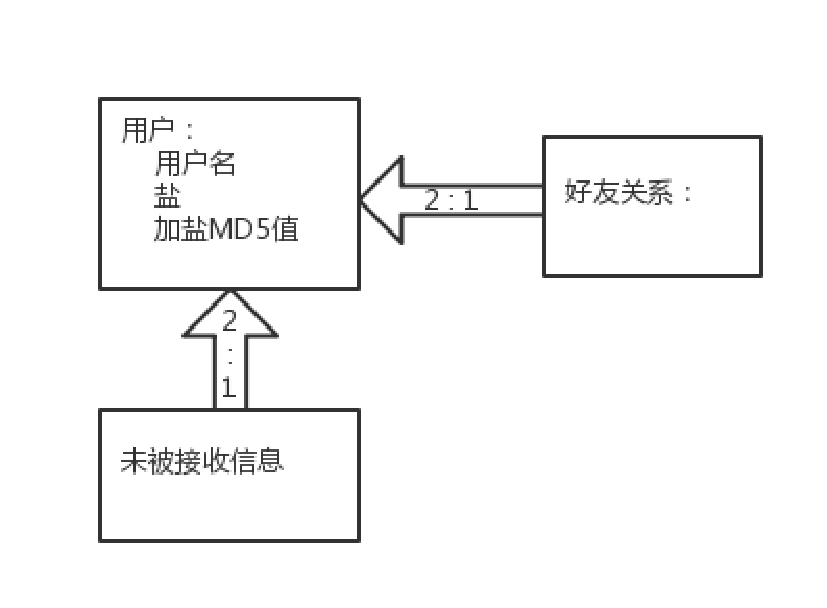
\includegraphics[width=10cm]{fig_db}
\end{figure}

\section{物理设计}
\subsection{数据库产品}
使用MySQL数据库。根据目前本软件的使用情况,一台云服务器已经可以很好地满足所有需求,所以没有采用分布式数据库。
\subsection{实体属性、类型、精度}
\subsubsection{客户数据表设计}
\begin{table}[htbp]
\centering
\caption{用户数据表Users设计} \label{tab:client-database}
\begin{tabular}{|c|c|c|c|c|}
    \hline
    字段名 & 类型 & 大小 & 说明 & 备注 \\
    \hline
    uname & varchar & 48 & 用户名 & 主键\\
    \hline
    md5 & char & 10 & 随机产生的加盐值 & ·\\
    \hline
    pw & char & 32 & 用户的登录密码加盐的MD5值 & · \\
    \hline
\end{tabular}
\note{用户数据表Users设计}
\end{table}

\subsubsection{联系人数据表设计}
\begin{table}[htbp]
\centering
\caption{联系人表Links设计} \label{tab:order-database}
\begin{tabular}{|c|c|c|c|c|}
    \hline
    字段名 & 类型 & 大小 & 说明 & 备注 \\
    \hline
    uname\_1 & varchar & 48 & 用户1 & 主键,外键,引用Users\\
    \hline
    uname\_2 & varchar & 48 & 用户2 & 主键,外键,引用Users \\
    \hline
\end{tabular}
\note{联系人表Links设计}
\end{table}
\section{安全性设计}
服务器调用数据库全部采用存储过程,不允许直接执行数据库语句,一般不会产生安全性问题。

\section{数据库管理与维护说明}
对于数据库的维护,随时对数据库中的信息加以调试和保存备份。同样需要个工作人员进行系统的分析和用户的反馈,对系统进行升级以及功能的完善。同时保证系统安全有序的运行。
\chapter{界面设计}
\section{服务器端界面}
服务器是命令行的,没有可见界面。

\section{登录界面}
\begin{figure}[h]
	\centering
	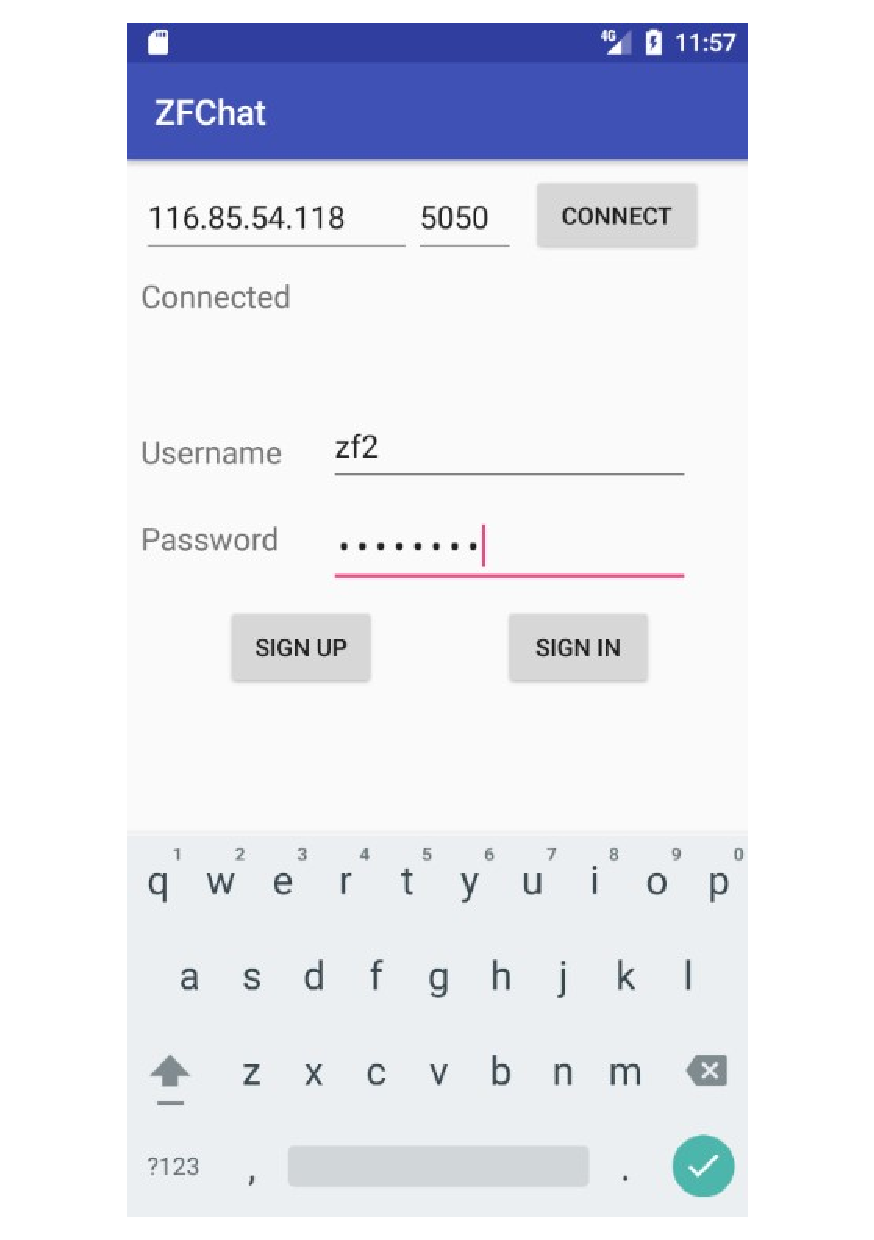
\includegraphics[width=10cm]{ui_signin}
\end{figure}

\section{联系人界面}
\begin{figure}[h]
	\centering
	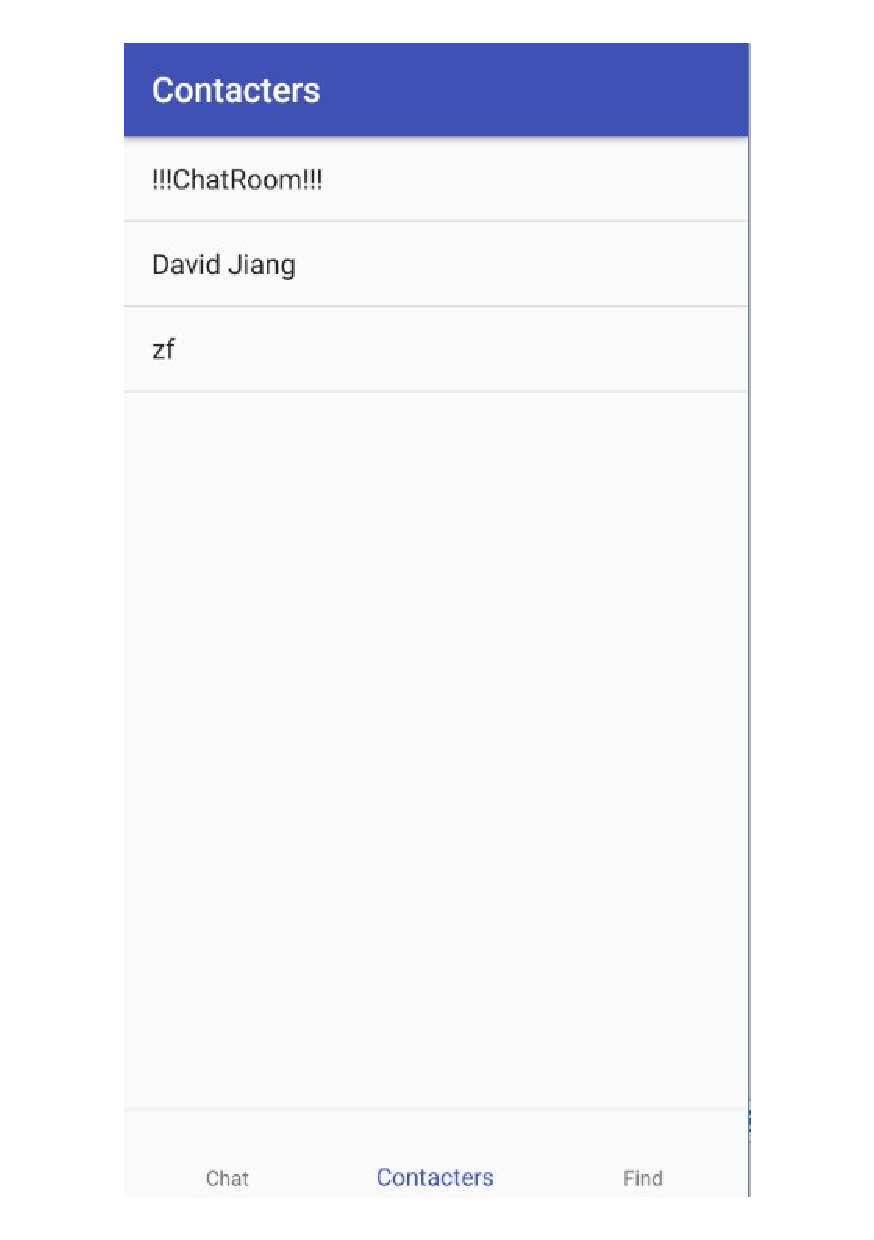
\includegraphics[width=10cm]{ui_contacters}
\end{figure}
\section{消息界面}
\begin{figure}[h]
	\centering
	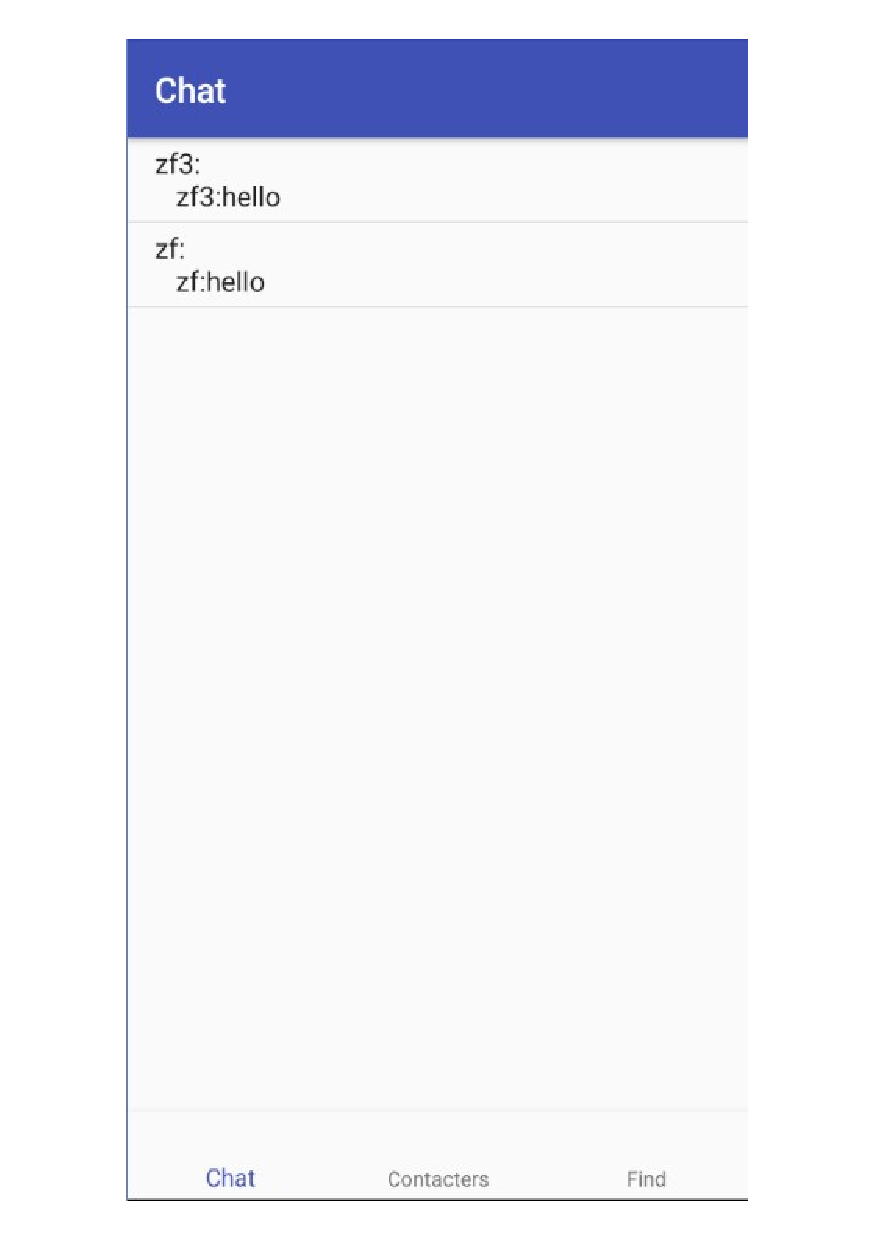
\includegraphics[width=10cm]{ui_chat}
\end{figure}
\section{聊天界面}
\begin{figure}[h]
	\centering
	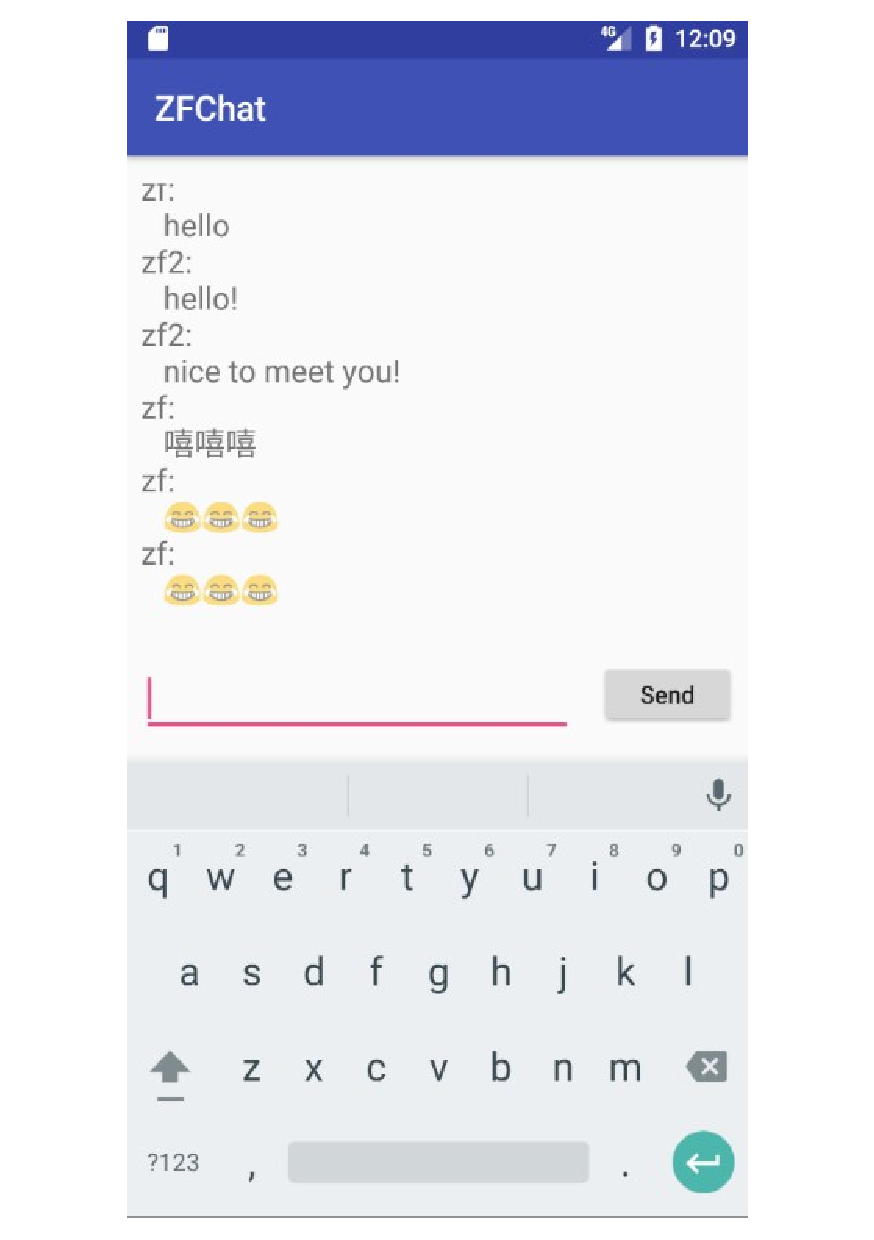
\includegraphics[width=10cm]{ui_message}
\end{figure}
\section{好友管理界面}
\begin{figure}[h]
	\centering
	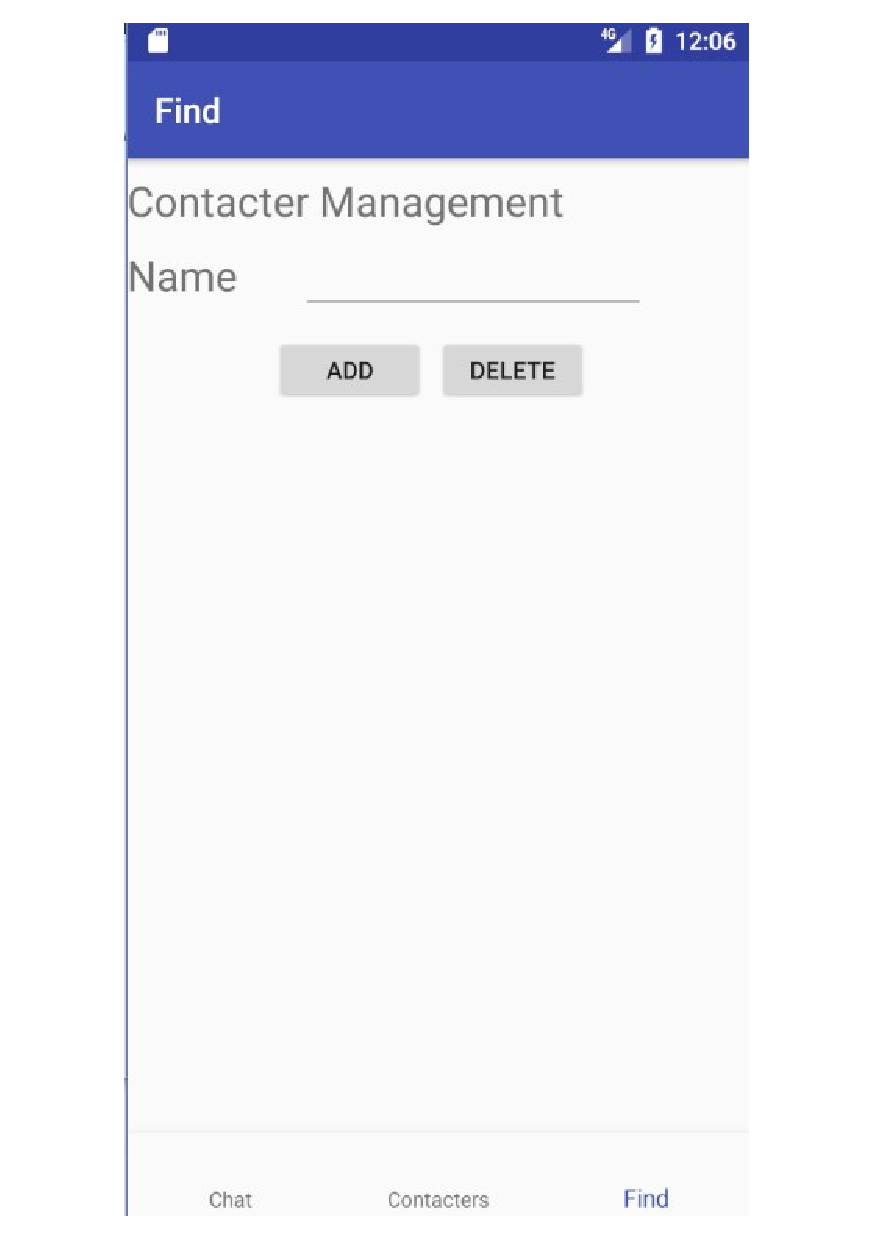
\includegraphics[width=10cm]{ui_find}
\end{figure}
\chapter{出错处理设计}
\section{数据库出错处理}
<<<<<<< HEAD
\subsection{事务故障}
如果出现事务故障,则遵循数据库系统设计的一般原则,找出并将故障事务从数据库中撤销。
\subsection{系统崩溃故障}
对于类似于停电,死机等系统崩溃故障,由于我们的数据库设计每次操作都会生成日志以及每周都会人工维护,故会尽可能恢复到故障前的样子。
\subsection{磁盘故障}
由于开发者资金紧缺,人手不足,如果出现了服务器上的磁盘故障,我们会在保障还能使用基本的聊天功能的情况下尝试恢复用户数据,但是完全丢失的数据无法由我们找回,只能由使用者将其重新恢复(如重新注册和原来一样的账号,重新添加原来的联系人)。
\subsection{不可抗力}
如果发生诸如地震火灾等不可抗力,我们只能十分遗憾地选择删库跑路。

\section{某模块失效处理}
大多数情况下我们都会提供聊天的功能,除非我们处于维护状态或出现了不可抗力,否则不会停止服务。

如果某版本的客户端出现bug,欢迎访问开发者论坛并提出,开发者会以最快的速度修复这个bug。
=======

\section{某模块失效处理}
如果服务器出现故障,重启一次。
>>>>>>> 29d41c134fbbe1596db211db949e2cd5634007bb

\chapter{安全保密设计}
可能的内容包括保密性、是否采取加密传输、密钥如何分发和管理等。
\chapter{维护设计}
可能的内容包括数据库的日常备份、压缩、维护等。

\chapter{图片}
本章展示图片相关用法。

\section{示例}
\begin{figure}[ht]
\centering

\includegraphics[width=10cm]{ustc_logo_fig}
\caption{测试图片} \label{fig:figure1}
\end{figure}

\section{带图注的图}
\begin{figure}[ht]
\centering

\includegraphics[width=10cm]{ustc_logo_fig}
\caption{带图注的图片}\label{fig:noted-figure}
\note{the solid lines represent the time histogram of the spontaneous activities of an old monkey cell(gray) and a young monkey cell (black). The bin-width is 1}
\end{figure}

\chapter{表格}

\section{A Simple Table}
\begin{table}[htbp]
\centering
\caption{这里是表的标题} \label{tab:simpletable}
\begin{tabular}{|c|c|}
    \hline
    a & b \\
    \hline
    c & d \\
    \hline
\end{tabular}
\note{这里是表的注释}
\end{table}

\section{长表格}
\begin{longtable}{ccc}
% 首页表头
\caption[长表格演示]{长表格演示} \label{tab:longtable} \\
\toprule[1.5pt]
名称  & 说明 & 备注\\
\midrule[1pt]
\endfirsthead
% 续页表头
\caption[]{长表格演示(续)} \\
\toprule[1.5pt]
名称  & 说明 & 备注 \\
\midrule[1pt]
\endhead
% 首页表尾
\hline
\multicolumn{3}{r}{\small 续下页}
\endfoot
% 续页表尾
\bottomrule[1.5pt]
\endlastfoot

AAAAAAAAAAAA   &   BBBBBBBBBBB   &   CCCCCCCCCCCCCC   \\
AAAAAAAAAAAA   &   BBBBBBBBBBB   &   CCCCCCCCCCCCCC   \\
AAAAAAAAAAAA   &   BBBBBBBBBBB   &   CCCCCCCCCCCCCC   \\
AAAAAAAAAAAA   &   BBBBBBBBBBB   &   CCCCCCCCCCCCCC   \\
AAAAAAAAAAAA   &   BBBBBBBBBBB   &   CCCCCCCCCCCCCC   \\
AAAAAAAAAAAA   &   BBBBBBBBBBB   &   CCCCCCCCCCCCCC   \\
AAAAAAAAAAAA   &   BBBBBBBBBBB   &   CCCCCCCCCCCCCC   \\
AAAAAAAAAAAA   &   BBBBBBBBBBB   &   CCCCCCCCCCCCCC   \\
AAAAAAAAAAAA   &   BBBBBBBBBBB   &   CCCCCCCCCCCCCC   \\
AAAAAAAAAAAA   &   BBBBBBBBBBB   &   CCCCCCCCCCCCCC   \\
AAAAAAAAAAAA   &   BBBBBBBBBBB   &   CCCCCCCCCCCCCC   \\
AAAAAAAAAAAA   &   BBBBBBBBBBB   &   CCCCCCCCCCCCCC   \\
AAAAAAAAAAAA   &   BBBBBBBBBBB   &   CCCCCCCCCCCCCC   \\
AAAAAAAAAAAA   &   BBBBBBBBBBB   &   CCCCCCCCCCCCCC   \\
AAAAAAAAAAAA   &   BBBBBBBBBBB   &   CCCCCCCCCCCCCC   \\
AAAAAAAAAAAA   &   BBBBBBBBBBB   &   CCCCCCCCCCCCCC   \\
AAAAAAAAAAAA   &   BBBBBBBBBBB   &   CCCCCCCCCCCCCC   \\
AAAAAAAAAAAA   &   BBBBBBBBBBB   &   CCCCCCCCCCCCCC   \\
AAAAAAAAAAAA   &   BBBBBBBBBBB   &   CCCCCCCCCCCCCC   \\
AAAAAAAAAAAA   &   BBBBBBBBBBB   &   CCCCCCCCCCCCCC   \\
AAAAAAAAAAAA   &   BBBBBBBBBBB   &   CCCCCCCCCCCCCC   \\
AAAAAAAAAAAA   &   BBBBBBBBBBB   &   CCCCCCCCCCCCCC   \\
AAAAAAAAAAAA   &   BBBBBBBBBBB   &   CCCCCCCCCCCCCC   \\
AAAAAAAAAAAA   &   BBBBBBBBBBB   &   CCCCCCCCCCCCCC   \\
AAAAAAAAAAAA   &   BBBBBBBBBBB   &   CCCCCCCCCCCCCC   \\
AAAAAAAAAAAA   &   BBBBBBBBBBB   &   CCCCCCCCCCCCCC   \\
AAAAAAAAAAAA   &   BBBBBBBBBBB   &   CCCCCCCCCCCCCC   \\
AAAAAAAAAAAA   &   BBBBBBBBBBB   &   CCCCCCCCCCCCCC   \\
AAAAAAAAAAAA   &   BBBBBBBBBBB   &   CCCCCCCCCCCCCC   \\
AAAAAAAAAAAA   &   BBBBBBBBBBB   &   CCCCCCCCCCCCCC   \\
AAAAAAAAAAAA   &   BBBBBBBBBBB   &   CCCCCCCCCCCCCC   \\
AAAAAAAAAAAA   &   BBBBBBBBBBB   &   CCCCCCCCCCCCCC   \\
AAAAAAAAAAAA   &   BBBBBBBBBBB   &   CCCCCCCCCCCCCC   \\
AAAAAAAAAAAA   &   BBBBBBBBBBB   &   CCCCCCCCCCCCCC   \\
AAAAAAAAAAAA   &   BBBBBBBBBBB   &   CCCCCCCCCCCCCC   \\
AAAAAAAAAAAA   &   BBBBBBBBBBB   &   CCCCCCCCCCCCCC   \\
\end{longtable}

\chapter{算法环境}
模板中使用 \texttt{algorithm2e} 宏包实现算法环境。关于该宏包的具体用法,
请阅读宏包的官方文档。

\begin{algorithm}[htbp]
\SetAlgoLined
\KwData{this text}
\KwResult{how to write algorithm with \LaTeX2e }

initialization\;
\While{not at end of this document}{
    read current\;
    \eIf{understand}{
        go to next section\;
        current section becomes this one\;
    }{
        go back to the beginning of current section\;
    }
}
\caption{算法示例1}
\label{algo:algorithm1}
\end{algorithm}

\IncMargin{1em}
\begin{algorithm}
\SetKwData{Left}{left}\SetKwData{This}{this}\SetKwData{Up}{up}
\SetKwFunction{Union}{Union}\SetKwFunction{FindCompress}{FindCompress}
\SetKwInOut{Input}{input}\SetKwInOut{Output}{output}

\Input{A bitmap $Im$ of size $w\times l$}
\Output{A partition of the bitmap}
\BlankLine
\emph{special treatment of the first line}\;
\For{$i\leftarrow 2$ \KwTo $l$}{
    \emph{special treatment of the first element of line $i$}\;
    \For{$j\leftarrow 2$ \KwTo $w$}{\label{forins}
        \Left$\leftarrow$ \FindCompress{$Im[i,j-1]$}\;
        \Up$\leftarrow$ \FindCompress{$Im[i-1,]$}\;
        \This$\leftarrow$ \FindCompress{$Im[i,j]$}\;
        \If(\tcp*[h]{O(\Left,\This)==1}){\Left compatible with \This}{\label{lt}
            \lIf{\Left $<$ \This}{\Union{\Left,\This}}
            \lElse{\Union{\This,\Left}}
        }
        \If(\tcp*[f]{O(\Up,\This)==1}){\Up compatible with \This}{\label{ut}
        \lIf{\Up $<$ \This}{\Union{\Up,\This}}
        \tcp{\This is put under \Up to keep tree as flat as possible}\label{cmt}
        \lElse{\Union{\This,\Up}}\tcp*[h]{\This linked to \Up}\label{lelse}
        }
    }
    \lForEach{element $e$ of the line $i$}{\FindCompress{p}}
}
\caption{算法示例2}\label{algo_disjdecomp}
\label{alog:algorithm2}
\end{algorithm}\DecMargin{1em}

\chapter{代码环境}
模板中使用 \texttt{listings} 宏包实现代码环境。详细用法见宏包的官方说明文档。

以下是代码示例,可以在文中任意位置引用\autoref{first-code} 。
\begin{lstlisting}[language=C, caption=示例代码, label={code:first-code}]
#include <stdio.h>

int main( )
{
    printf("hello, world\n");
    return 0;
}
\end{lstlisting}

\chapter{引用文献标注}

\section{著者-出版年制标注法}

\noindent
\verb|\citestyle{ustcauthoryear}|
\citestyle{ustcauthoryear}

\noindent
\begin{tabular}{l@{\quad$\Rightarrow$\quad}l}
  \verb|\cite{knuth86a}| & \cite{knuth86a}\\
  \verb|\citet{knuth86a}| & \citet{knuth86a}\\
  \verb|\citet[chap.~2]{knuth86a}| & \citet[chap.~2]{knuth86a}\\[0.5ex]
  \verb|\citep{knuth86a}| & \citep{knuth86a}\\
  \verb|\citep[chap.~2]{knuth86a}| & \citep[chap.~2]{knuth86a}\\
  \verb|\citep[see][]{knuth86a}| & \citep[see][]{knuth86a}\\
  \verb|\citep[see][chap.~2]{knuth86a}| & \citep[see][chap.~2]{knuth86a}\\[0.5ex]
  \verb|\citet*{knuth86a}| & \citet*{knuth86a}\\
  \verb|\citep*{knuth86a}| & \citep*{knuth86a}\\
\end{tabular}

\noindent
\begin{tabular}{l@{\quad$\Rightarrow$\quad}l}
  \verb|\citet{knuth86a,tlc2}| & \citet{knuth86a,tlc2}\\
  \verb|\citep{knuth86a,tlc2}| & \citep{knuth86a,tlc2}\\
  \verb|\cite{knuth86a,knuth84}| & \cite{knuth86a,knuth84}\\
  \verb|\citet{knuth86a,knuth84}| & \citet{knuth86a,knuth84}\\
  \verb|\citep{knuth86a,knuth84}| & \citep{knuth86a,knuth84}\\
\end{tabular}

\section{顺序编码制标注法}

\noindent
\verb|\citestyle{ustcnumerical}|
\citestyle{ustcnumerical}

\noindent
\begin{tabular}{l@{\quad$\Rightarrow$\quad}l}
  \verb|\cite{knuth86a}| & \cite{knuth86a}\\
  \verb|\citet{knuth86a}| & \citet{knuth86a}\\
  \verb|\citet[chap.~2]{knuth86a}| & \citet[chap.~2]{knuth86a}\\[0.5ex]
  \verb|\citep{knuth86a}| & \citep{knuth86a}\\
  \verb|\citep[chap.~2]{knuth86a}| & \citep[chap.~2]{knuth86a}\\
  \verb|\citep[see][]{knuth86a}| & \citep[see][]{knuth86a}\\
  \verb|\citep[see][chap.~2]{knuth86a}| & \citep[see][chap.~2]{knuth86a}\\[0.5ex]
  \verb|\citet*{knuth86a}| & \citet*{knuth86a}\\
  \verb|\citep*{knuth86a}| & \citep*{knuth86a}\\
\end{tabular}

\noindent
\begin{tabular}{l@{\quad$\Rightarrow$\quad}l}
  \verb|\citet{knuth86a,tlc2}| & \citet{knuth86a,tlc2}\\
  \verb|\citep{knuth86a,tlc2}| & \citep{knuth86a,tlc2}\\
  \verb|\cite{knuth86a,knuth84}| & \cite{knuth86a,knuth84}\\
  \verb|\citet{knuth86a,knuth84}| & \citet{knuth86a,knuth84}\\
  \verb|\citep{knuth86a,knuth84}| & \citep{knuth86a,knuth84}\\
  \verb|\cite{knuth86a,knuth84,tlc2}| & \cite{knuth86a,knuth84,tlc2}\\
\end{tabular}

\section{其他形式的标注}

\noindent
\begin{tabular}{l@{\quad$\Rightarrow$\quad}l}
  \verb|\citealt{tlc2}| & \citealt{tlc2}\\
  \verb|\citealt*{tlc2}| & \citealt*{tlc2}\\
  \verb|\citealp{tlc2}| & \citealp{tlc2}\\
  \verb|\citealp*{tlc2}| & \citealp*{tlc2}\\
  \verb|\citealp{tlc2,knuth86a}| & \citealp{tlc2,knuth86a}\\
  \verb|\citealp[pg.~32]{tlc2}| & \citealp[pg.~32]{tlc2}\\
  \verb|\citenum{tlc2}| & \citenum{tlc2}\\
  \verb|\citetext{priv.\ comm.}| & \citetext{priv.\ comm.}\\
\end{tabular}

\noindent
\begin{tabular}{l@{\quad$\Rightarrow$\quad}l}
  \verb|\citeauthor{tlc2}| & \citeauthor{tlc2}\\
  \verb|\citeauthor*{tlc2}| & \citeauthor*{tlc2}\\
  \verb|\citeyear{tlc2}| & \citeyear{tlc2}\\
  \verb|\citeyearpar{tlc2}| & \citeyearpar{tlc2}\\
\end{tabular}

\bibliography{bib/tex}


\end{document}
